\chapter{Experimenty DOSIS a DOSIS 3D}
Informace v tomto oddíle byly čerpány ze zdrojů \cite{dosis,dosis2}.

Experimenty Evropské kosmické agentury DOSIS (Dose Distribution Inside the ISS, distribuce dávky uvnitř ISS) a DOSIS 3D probíhají roku 2009 za účelem vyšetření prostorové distribuce dávky v modulu ISS Columbus. Kýženým cílem bylo získání dat, která by vedla k vytvoření 3D modelu této distribuce.

Měření byla, respektive jsou prováděna pasivními a aktivními detektory, které jsou pevně umístěny v modulu Columbus. Pasivní detektory zajišťovaly určení prostorové distribuce dávky a dlouhodobého vývoje pole záření, aktivní naopak sloužily k určení časové závislosti pole záření. V případě aktivních detektorů se jednalo o dva detektory DOSTEL (DOSimetry TELescope). V dalším textu se budeme zabývat pouze pasivními detektory.

\section{Rozmístění pasivních detektorů}
V rámci experimentu DOSIS, resp. DOSIS3D bylo v modulu Columbus rozmístěno jedenáct PDPs (Passive Detector Packages, balíčky pasivních dektorů), které obsahovaly termoluminiscenční detektory (TLD), opticky stimulované luminiscenční detektory (OSLD) a detektory stop v pevné fázi (CR-39). Na obr. \ref{fig:Columbus_rozmisteni} vidíme rozmístění PDPs; pět z nich je umístěno na čelní stěně, dalších šest na zadní stěně. Jedenáctý balíček označený symbolem X, též označovaný jako Triple PDP (trojitý PDP), je umístěn blízko aktivních detektorů a pokrývá větší plochu než ostatní PDPs. Osm PDPs je umístěno ve skříňových modulech (viz oddíl \ref{sec:ISS_columbus}); více informací o umístění pasivních detektorů je k dostání v \cite{dosis}. %další obrázek???
\begin{figure}[H]
  \centering
  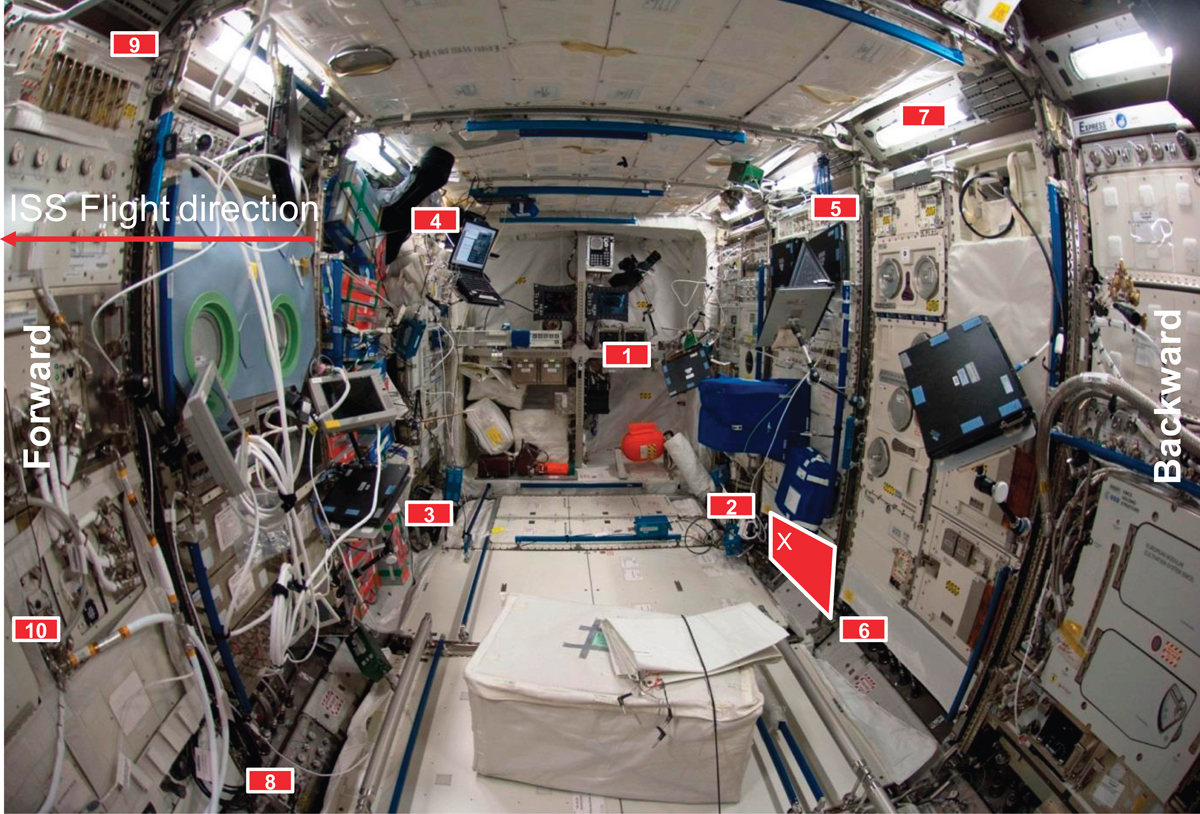
\includegraphics[width=\textwidth]{columbus_rozmisteni.jpg}
  \caption{Rozmístění jedenácti balíčků s pasivními detektory v modulu Columbus; jedenáctý je označen symbolem X a v jeho blízkosti jsou umístěny i aktivní detektory. Obrázek dále obsahuje šipku ukazující směr letu. \cite{dosis}}
  \label{fig:Columbus_rozmisteni}
\end{figure}

\section{Průběh experimentu}
Experiment DOSIS probíhal mezi lety 2009 a 2011. Doba trvání experimentu DOSIS3D byla původně stanovena na rozmezí let 2012-2016, avšak v roce 2016 byla prodloužena a experiment stále běží. V rámci těchto experimentů bylo v modulu Columbus postupně upevněno 8 sad pasivních detektorů (DOSIS -- dvě sady, DOSIS3D -- šest sad). Každá sada obsahovala obsahovala výše zmíněných 11 PDPs. V tab. \ref{tab:timeline} je vidět časový vývoj v obměně těchto sad a aktivních detektorů (ty byly pouze dva), tab. \ref{tab:timeline_passive} pak obsahuje podrobnější informace o pasivních detektorech (dopravení na ISS, instalaci, doba používání, ukončení měření, návrat na Zem, nadmořská výška). První z experimentů započal 15. července 2009 startem raketoplánu Endeavor, na jehož palubě byla
první sada pasivních detektorů spolu s aktivním detektorem DOSTEL-1. Jeho část skládající se z měření pasivními detektory skončila 26. května 2010 návratem druhé sady. Experiment DOSIS3D započal 15. května 2012 startem lodi Soyuz 30S. 
\begin{table}[H]
  \centering
  \caption{Vývoj experimentů DOSIS a DOSIS3D v čase. Číslo na svislé ose označuje $n$-tou sadu pasivních detektorů, písmeno A značí aktivní detektor. \cite{dosis}}
  \label{tab:timeline}
  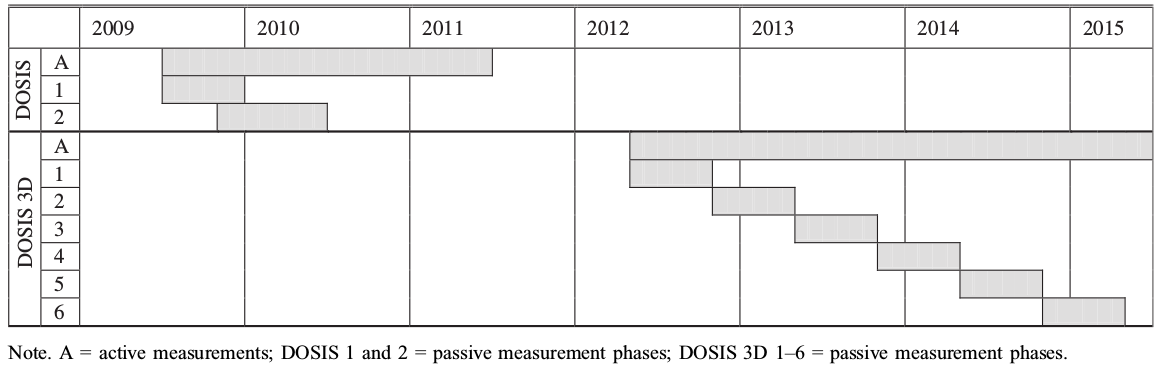
\includegraphics[width=\textwidth]{dosis_timeline}
\end{table}
\begin{table}[H]
  \centering
  \caption{Podrobný časový vývoj používaných sad pasivních detektorů (Phase). Tabulka dále obsahuje poměr doby měření a času, který detektor strávil na ISS (v procentech) a také nadmořskou výšku ISS pro každou sadu. \cite{dosis}}
  \label{tab:timeline_passive}
  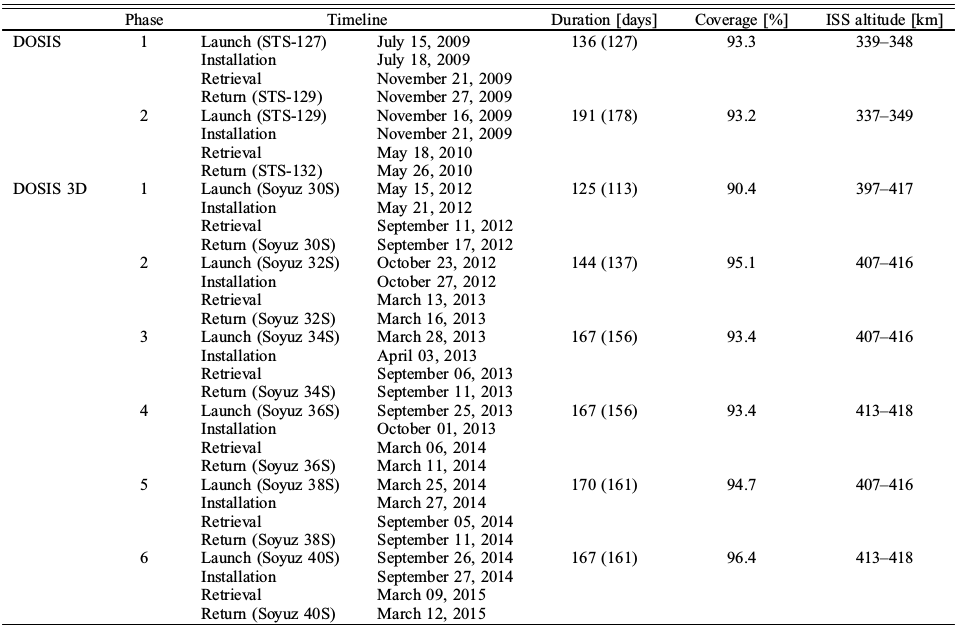
\includegraphics[width=\textwidth]{dosis_timeline_passive}
\end{table}

\subsection{Vývoj nadmořské výšky a solárního cyklu} %špatné odsazení
Naměřená data jsou ovlivněna řadou parametrů. Nadmořská výška a fáze solárního cyklu jsou jedny z nejvýznamnějších. 

Na obr. \ref{subfig:dosis_altitude} je znázorněn časový vývoj nadmořské výšky ISS. Pro DOSIS nadmořská výška nabývala hodnot z intervalu [337, 375] km, pro DOSIS3D nabývala hodnot z intervalu [398, 417] km. V obrázku lze vypozorovat prudký nárůst z cca 340 km do 375 km, který se udál ke konci experimentu DOSIS; tehdy již měřily pouze aktivní detektory. Změna nadmořské výšky ovlivňuje ozáření stanice (viz oddíl \ref{sec:kosmickeZareni_altitude}). 

Z informací v oddílu \ref{sec:kosmickeZareni_solar} plyne, že za solárního maxima je obdržená dávka nejmenší a naopak za solárního minima největší (za předpokladu stálosti ostatních parametrů ovlivňujících velikost obdržené dávky). To je znázorněno na obr. \ref{subfig:dosis_solarCycle}, kde je zobrazena závislost četnosti detekovaných neutronů na čase. Experiment DOSIS probíhal za slunečního minima (2009 až 2011) a naopak experiment DOSIS3D probíhal za solárního maxima, které nastalo v letech 2013 a 2014.   
\begin{figure}[h]
  \centering
  \begin{subfigure}{0.45\textwidth}
    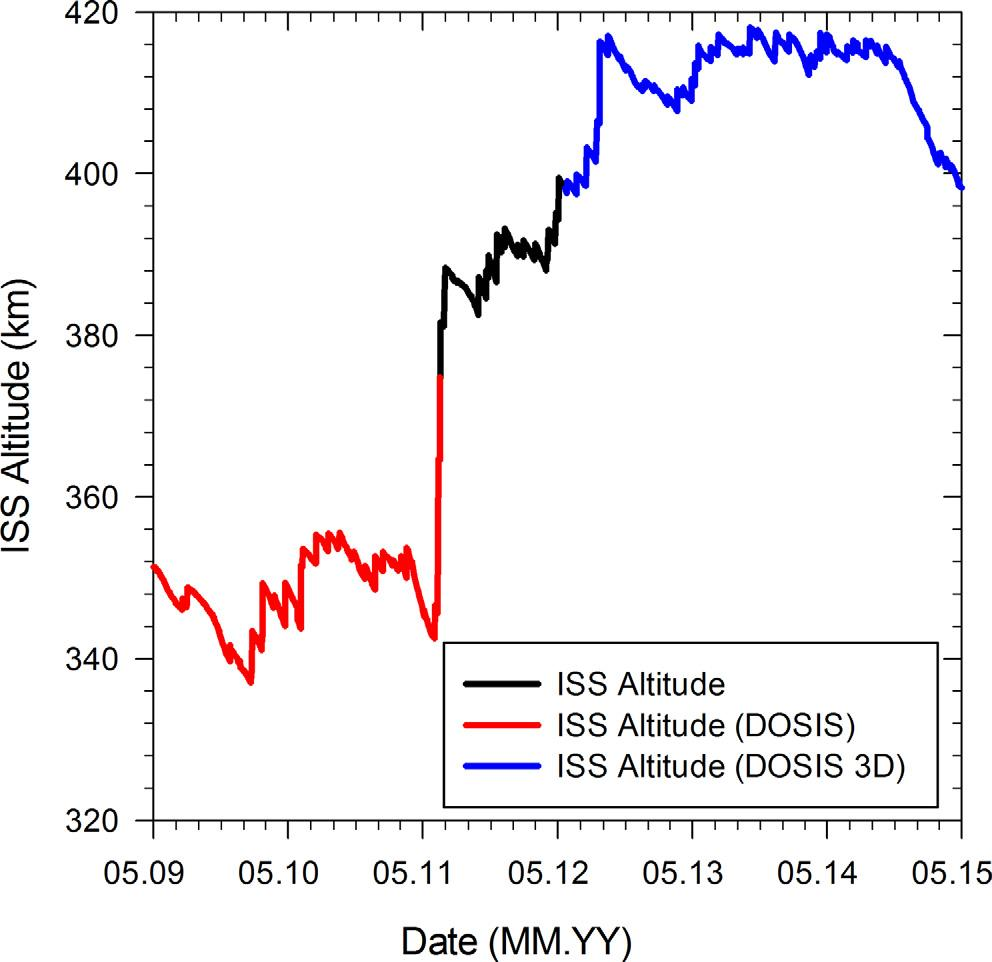
\includegraphics[width=\textwidth]{dosis_altitude.jpeg}
    \caption{}
    \label{subfig:dosis_altitude}
  \end{subfigure}
  \begin{subfigure}{0.45\textwidth}
    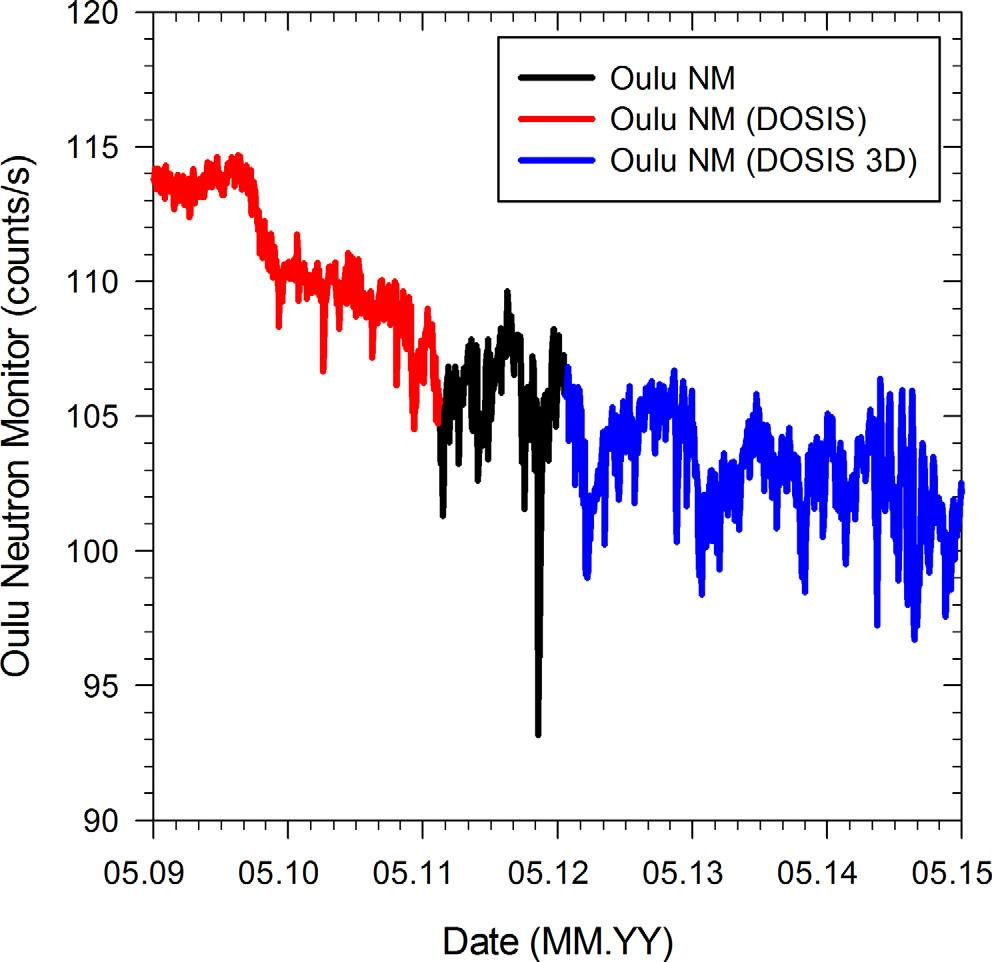
\includegraphics[width=\textwidth]{dosis_solarCycle.jpeg}
    \caption{}
    \label{subfig:dosis_solarCycle}
  \end{subfigure}
  \caption{V (a) je časový vývoj nadmořské výšky ISS: červeně je vyznačen vývoj v rámci DOSIS, modře v rámci DOSIS3D; černě je označen vývoj nadmořské výšky v době, kdy neprobíhal žádný z experimentů. V (b) je naměřená četnost Oulu neutronovým monitorem, značení je stejné jako v (a). \cite{dosis}} 
  \label{fig:dosis_parameters}
\end{figure}


%Nevýhodou pasivních detektorů je skutečnost, že po každém měření musely být dopraveny zpět na Zem do příslušné laboratoře a teprve tam byly vyhodnoceny; avšak oproti aktivním detektorům nemusejí být napájeny proudem, což je v prostředí ISS velmi praktické. 



